\documentclass[a4paper, 11pt]{article}
\usepackage{lmodern}
\usepackage[svgnames]{xcolor} % Required to specify font color
\input{/home/aroquemaurel/cours/includesLaTeX/couleurs.tex}

\usepackage[utf8]{inputenc}
\usepackage[T1]{fontenc}
\usepackage[francais]{babel}
\usepackage[top=1.7cm, bottom=1.7cm, left=1.7cm, right=1.7cm]{geometry}
\usepackage{verbatim}
\usepackage[urlbordercolor={1 1 1}, linkbordercolor={1 1 1}, linkcolor=vert1, urlcolor=bleu, colorlinks=true]{hyperref}
\usepackage{tikz} %Vectoriel
\usepackage{listings}
\usepackage{fancyhdr}
\usepackage{multido}
\usepackage{amssymb}
\usepackage{float}
\usepackage{graphicx} % Required for box manipulation

\newcommand{\titre}{Gestionnaire des bulletins d'un établissement}
\newcommand{\subtitle}{DM \no{}1}
\newcommand{\auteur}{Antoine de \bsc{Roquemaurel}}
\newcommand{\formation}{L3 Informatique}
\newcommand{\semestre}{6}
\newcommand{\prof}{}
\newcommand{\numero}{1}
\newcommand{\typeDoc}{DM}
\newcommand{\module}{Programmation événementielle}


\newcommand{\pole}{}
\newcommand{\sigle}{pge}
\input{/home/aroquemaurel/cours/includesLaTeX/listings.tex} %prise en charge du langage algo
\input{/home/aroquemaurel/cours/includesLaTeX/l3/tddm.tex}
\input{/home/aroquemaurel/cours/includesLaTeX/l3/remarquesExempleAttention.tex}
\input{/home/aroquemaurel/cours/includesLaTeX/polices.tex}
\input{/home/aroquemaurel/cours/includesLaTeX/affichageChapitre.tex}
\input{/home/aroquemaurel/cours/includesLaTeX/couverture.tex}
\makeatother

\begin{document}
	\maketitle
	\section*{Avant-propos}
	Ce rapport contient les choix d'implémentation et de conception pour un projet dans le cadre de la L3 Informatique parcours Ingénierie des Systèmes
	Informatiques de l'université Toulouse III -- Paul Sabatier.
	Il s'agit d'un logiciel permettant la gestion des bulletins d'un établissement scolaire.

	Celui-ci doit être développé en Java en utilisant la bibliothèque graphique \texttt{Swing}, ceci à l'aide de l'éditeur WYSIWYG Matisse présent dans
	\textit{Netbeans}. Ci-joint à ce rapport est donc présent les sources du logiciel sous forme de projet Netbeans.

	\section{Conception}
		L'application à été conçue en différents packages afin de faciliter le développement et la relecture du code. Cette répartition à été fait en deux
		packages principaux : les données dites << métiers >>, et l'interface graphique. 
		
		Ainsi, au besoin il est tout à fait possible de ne changer que l'interface de notre programme. 

		\begin{figure}[H]
			\hspace{-36px}
			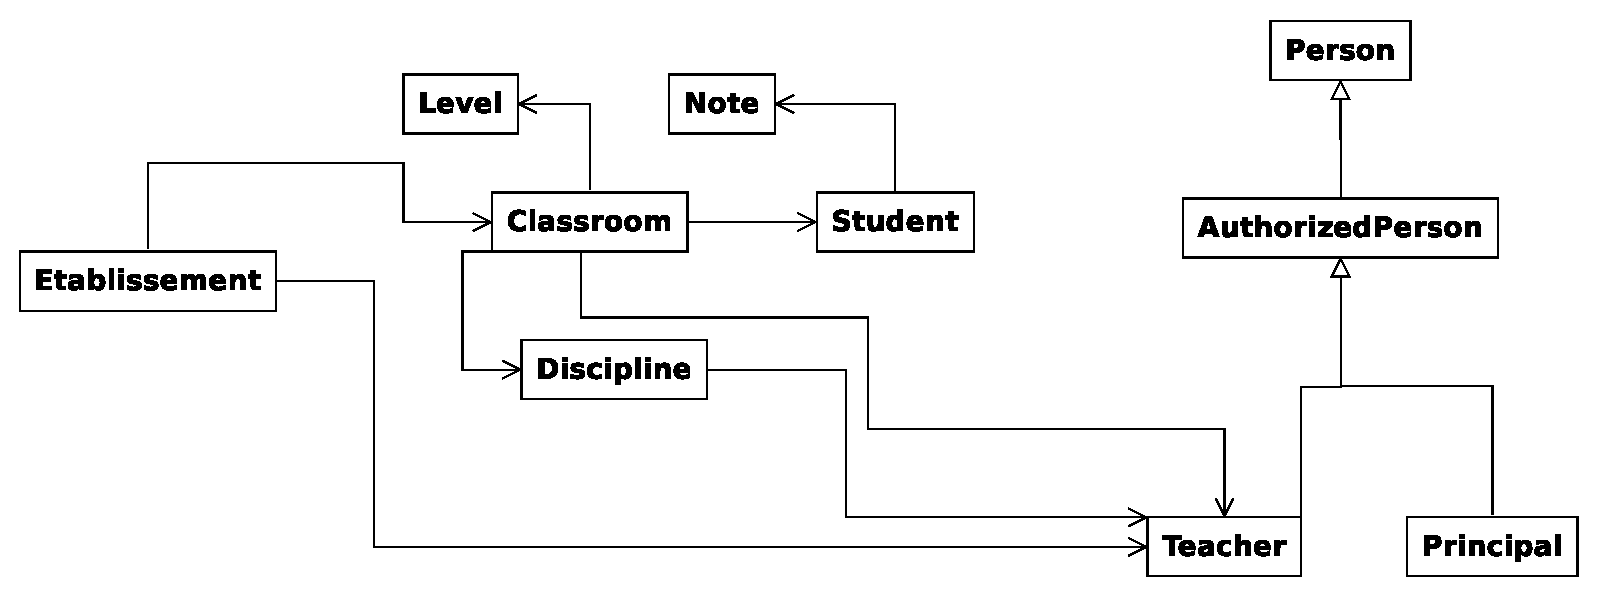
\includegraphics[width=20cm]{Diagramme1.eps}
			\caption{Diagramme de classe des données métiers}
			\label{fig:diagClasse}
		\end{figure}

		\subsection{Répartition en package}
		Notre application utilise un assez grand nombre de package afin de découper au mieux le problème, nous allons voir ici comment les fichiers sont
		organisés.

		\subsubsection{Données métiers}
		Les données de l'application, indépendamment de l'interface.
		\begin{description}
			\item[\texttt{etablissement}] Les données concernant l'établissement.
			\item[\texttt{etablissement.classroom}] Tout ce qui concerne une classe, les notes, le niveau, \ldots
			\item[\texttt{etablissement.person}] Toutes les personnes 
		\end{description}

		\subsubsection{Interface Graphique Swing}
			\paragraph{Lancement de l'interface} C'est le package racine, permettant de lancer la fenêtre principale et les principaux panneaux.
			\paragraph{Gestion des données} Ce package contient des sous-package permettant de gérer les données, c'est-à-dire, les vues, les modèles et les éditeurs.

		\begin{description}
			\item[\texttt{gui.data.editors}] Classes \texttt{editors}
			\item[\texttt{gui.data.models}] Classes modèles 
			\item[\texttt{gui.data.renderer}] Classes de vues 
		\end{description}
		\paragraph{Images}
		Celui-ci ne contient que les images permettant d'afficher des icônes dans les boutons.
		\paragraph{Panneau du directeur}
		Contient toutes les fenêtres et panneaux permettant l'utilisation du logiciel connecté en tant que principal.
		\begin{description}
			\item[\texttt{gui.principal}] Panneau principal
			\item[\texttt{gui.principal.classrooms}] Gestion des classes
			\item[\texttt{gui.principal.teachers}] Gestion des professeurs
		\end{description}

		\paragraph{Panneau des professeur}
		De la même manière que le package du principal, celui-ci gère les professeurs.

		\subsection{Connexion avec l'IHM}
		Afin de simplifier au maximum le problème, je suis partis du principe que l'interface Swing ne peut lancer qu'un seul jeu de données simultanément, ainsi
		la création de plusieurs instance de \texttt{MainFrame} pourrait empêcher le bon fonctionnement du programme.

		\begin{remarque}
			Il aurait pus être intéressant de transformer la classe \texttt{MainFrame} en singleton, cela n'a pas été fait car cela ne fait pas l'objet du cours
			et n'est pas indispensable
		\end{remarque}

		La classe MainFrame, contient plusieurs attributs statiques, avec ces données, on peut obtenir toutes les informations métiers et les modifier très
		facilement.

		L'attribut \texttt{\_etablissement} contient toutes les données de l'application, comme le montre le diagramme de classe figure \ref{fig:diagClasse}. \\
		Le second attribut intéressant est \texttt{\_currentPerson}, c'est la personne qui s'est connecté, ça permet d'afficher des informations différentes en
		fonction de l'utilisateur.

		\subsection{Utilisation des collection Java}
		Afin d'avoir un système le plus efficace est robuste possible, j'ai utilisé plusieurs types de collections, particulièrement pour aider à un trie
		efficace grâce au \texttt{TreeSet}, mais également grâce à une \texttt{Map} liant une matière à une note : celle-ci sont présente chez l'élève.

	\section{Choix d'interface}
	Le développement de l'interface s'est effectuée en respectant ce qui était demandé dans le sujet, ainsi peu de liberté ont été prise afin de satisfaire au
	maximum la demande.

	Des contrôles ont été fait au niveau de l'insertion des notes : une note doit être entre 0 et 20, ce contrôle s'effectue à l'aide d'un \textit{spinner}.
	\section{Données de tests}
	Afin de pouvoir tester le logiciel dans de bonnes conditions, des données de tests sont insérés au lancement du logiciel. Pour cela, il faut
	exécuter la méthode \texttt{main} présent dans le package \texttt{managementStudent}. Celle-ci va insérer automatiquement un proviseur, des
	professeurs, des classes avec leurs élèves associés ainsi que des notes : Toutes les données de lectures peuvent être essayés, il est ensuite
	possible d'ajouter et d'éditer des données depuis le logiciel.

	\begin{remarque}
		Il n'était demandé aucune sérialisation ou stockage des données dans une base de données, ainsi une fois le logiciel fermée, toutes les données
		sont définitivement perdues. Le lancement du logiciel réinsèrera le jeu d'essais.

		Il aurait été possible de stocker les données à l'aide d'une base \textit{Sqlite} afin d'avoir la puissance et la souplesse des bases de
		données, ou une simple sérialisation de nos objets aurait pu faire l'affaire: ces deux solutions ont l'avantage d'être rapide à mettre en place.
	\end{remarque}
\end{document}


